\documentclass[../AnalisiDeiRequisiti.tex]{subfiles}
\begin{document}
	\section{Appendice A: Hex}

	\subsection{Il gioco}
		Hex è un gioco da tavolo inventato dal matematico danese Piet Hein nel 1942, e reinventato indipendentemente dal futuro premio Nobel per l'economia statunitense John Nash nel 1948.
		
		In una scacchiera romboidale con caselle esagonali, i due giocatori devono disporre le proprie pedine in modo da formare una linea continua tra i due lati opposti del proprio colore (ogni giocatore ha due lati del rombo, non contigui).
		La scacchiera può essere di dimensione 10x10, 11x11 o 14x14.
		I giocatori hanno due colori, di solito rosso e blu. Alternatamente pongono una pedina in una casella esagonale della scacchiera. L'obiettivo del giocatore rosso è di formare una linea continua che connette i due lati rossi della scacchiera, l'obiettivo del giocatore blu è connettere i lati blu.
		
		\begin{figure}
			\centering
			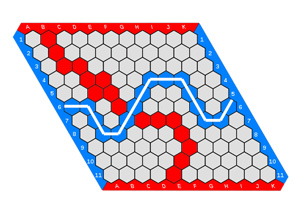
\includegraphics{./Figures/HexBoard.jpg}
			\caption{Esempio di partita a Hex}\label{fig:1}
		\end{figure}
	
	\subsection{Specifiche}
		Nel Capitolato d'appalto il \proponente\ desidera che venga scritta una versione di Hex tramite l'editor di diagrammi UML SweDesigner.
		
		Il gruppo \kaleidoscode\ intende produrre una versione di Hex che permetta di giocare in modalità \textit{pvp} tra due giocatori in tutte e tre le possibili scacchiere.
		È un requisito desiderabile per il gruppo creare un piccolo menù che permetta di scegliere la scacchiera e altre funzionalità di base come un regolamento.
		
		
		%NOTA A PIE DI PAGINA^ a b c d Martin Gardner, Hexaflexagons and Other Mathematical Diversions: The First Scientific American Book of Puzzles and Games, University of Chicago Press, 1988, p. 75, ISBN 978-0-226-28254-1.
	
	
\end{document}